\documentclass[preprint, 12pt]{elsarticle}
\usepackage{chemfig}
\usepackage{tikz}
\usepackage{graphicx}
\usepackage{amsmath, amssymb}
\setlength{\parindent}{0pt}
\usepackage{pgfplots}
\pgfplotsset{
	compat=1.3,
}
\pgfplotscreateplotcyclelist{line styles}{
	black,solid\\
	blue,dashed\\
	red,dotted\\
	orange,dashdotted\\
}

\newcommand*\GnuplotDefs{
	% set number of samples
	set samples 50;
	%
	%%% from <https://en.wikipedia.org/wiki/Normal_distribution>
	% cumulative distribution function (CDF) of normal distribution
	cdfn(x,mu,sd) = 0.5 * ( 1 + erf( (x-mu)/sd/sqrt(2)) );
	% probability density function (PDF) of normal distribution
	pdfn(x,mu,sd) = 1/(sd*sqrt(2*pi)) * exp( -(x-mu)^2 / (2*sd^2) );
	% PDF of a truncated normal distribution
	tpdfn(x,mu,sd,a,b) = pdfn(x,mu,sd) / ( cdfn(b,mu,sd) - cdfn(a,mu,sd) );
}
\usepackage{geometry}
\usepackage{mathtools}
\usepackage{tkz-berge}
\usetikzlibrary{automata}
\usetikzlibrary{arrows}
\usetikzlibrary{positioning,shapes,shadows,arrows}
\usetikzlibrary{shapes.geometric}
\usetikzlibrary{calendar,shadings}
\renewcommand*{\familydefault}{\sfdefault}
\colorlet{winter}{blue}
\colorlet{spring}{green!60!black}
\colorlet{summer}{orange}
\colorlet{fall}{red}
\newcount\mycount

\newcommand\shapeLarge{50mm}
\newcommand\shapeMedium{25mm}
\newcommand\shapeSmall{5mm}

\newcommand*{\xMin}{0}%
\newcommand*{\xMax}{6}%
\newcommand*{\yMin}{0}%
\newcommand*{\yMax}{6}%
\newcommand*{\zMax}{6}%
\newcommand*{\zMin}{0}%

\definecolor{colorwaveA}{RGB}{98,145,224}
\definecolor{colorwaveB}{RGB}{250,250,50}
\definecolor{colorwaveC}{RGB}{25,125,25}
\definecolor{colorwaveD}{RGB}{100,100,100}
\definecolor{colorwaveE}{RGB}{80,100,1}
\definecolor{colorwaveF}{RGB}{60,1,1}
\definecolor{colorwaveG}{RGB}{25,1,100}
\definecolor{colorwaveH}{RGB}{1,90,1}
\definecolor{colorwaveI}{RGB}{1,100,1}
\definecolor{colorwaveJ}{RGB}{1,1,1}


\tikzset{%
	shapeTriangle/.style={draw,shape=regular polygon,fill=colorwaveA,circular drop shadow,regular polygon sides=3,minimum size=\shapeSmall,inner sep=0pt,outer sep=0pt},
	shapeTriangle3/.style={shapeTriangle,fill=colorwaveD,circular drop shadow,shape border rotate=45},
	shapeTriangle4/.style={shapeTriangle,fill=colorwaveA,circular drop shadow,shape border rotate=90},
	shapeTriangle5/.style={shapeTriangle,fill=colorwaveB,shape border rotate=135},
	shapeTriangle6/.style={shapeTriangle,fill=colorwaveC,shape border rotate=180},
	shapeTriangle7/.style={shapeTriangle,fill=colorwaveE,shape border rotate=225},
	shapeTriangle8/.style={shapeTriangle,fill=colorwaveF,shape border rotate=270},
	shapeTriangle9/.style={shapeTriangle,fill=colorwaveG,shape border rotate=315},
}

\tikzset{%
	shapeUgaritic/.style={draw,shape=regular polygon,fill=colorwaveD,circular drop shadow,regular polygon sides=3,minimum size=\shapeSmall,inner sep=0pt,outer sep=0pt},
}

\tikzset{%
	shapeSquare/.style={draw,shape=regular polygon,fill=colorwaveC,circular drop shadow,regular polygon sides=4,minimum size=\shapeSmall,inner sep=0pt,outer sep=0pt},
	shapeSquare2/.style={shapeSquare,shape border rotate=45},
}

\tikzset{%
	shapeHexagon/.style={draw,shape=regular polygon,fill=colorwaveA,circular drop shadow,regular polygon sides=6,minimum size=\shapeSmall,inner sep=0pt,outer sep=0pt},
	shapeHexagon2/.style={shapeHexagon,shape border rotate=90},
}

\tikzset{%
	shapeOctagon/.style={draw,shape=regular polygon,fill=colorwaveB,circular drop shadow,regular polygon sides=8,minimum size=\shapeSmall,inner sep=0pt,outer sep=0pt},
	shapeOctagon2/.style={shapeHexagon,shape border rotate=45},
}
\tikzset{%
	shapeEllipse/.style={draw,shape=ellipse,minimum size=\shapeSmall,inner sep=0pt,outer sep=0pt},
	shapeEllipse2/.style={shapeEllipse,shape border rotate=90},
}

\tikzset{%
	closedFigure/.style={draw=\draw[->,rounded corners=0.2cm,shorten >=2pt]
		(1.5,0.5)-- ++(0,-1)-- ++(1,0)-- ++(0,2)-- ++(-1,0)-- ++(0,2)-- ++(1,0)--
		++(0,1)-- ++(-1,0)-- ++(0,-1)-- ++(-2,0)-- ++(0,3)-- ++(2,0)-- ++(0,-1)--
		++(1,0)-- ++(0,1)-- ++(1,0)-- ++(0,-1)-- ++(1,0)-- ++(0,-3)-- ++(-2,0)--
		++(1,0)-- ++(0,-3)-- ++(1,0)-- ++(0,-1)-- ++(-6,0)-- ++(0,3)-- ++(2,0)--
		++(0,-1)-- ++(1,0)}
}

\tikzstyle{start}=[circle, draw=none,,minimum size=\shapeMedium, fill=blue, circular drop shadow,text centered, anchor=north, text=white]
\tikzstyle{finish}=[circle, draw=none,,minimum size=\shapeMedium, fill=blue,circular drop shadow,text centered, anchor=north, text=white]
\tikzstyle{finish}=[rectangle, draw=none, ,minimum size=\shapeMedium,fill=blue,circular drop shadow,text centered, anchor=north, text=white]

\usepackage[noadjust]{cite}
\usepackage{algpseudocode}
\usepackage{listings}
\usepackage{algorithm}
\usepackage{color}
\usepackage{parskip}
\usepackage{amsfonts}
\usepackage{amsthm}
\usepackage{tikz}
\usepackage{tkz-berge}
\usepackage{caption}
\usepackage{hyperref}
\usepackage{amsrefs}
\usepackage{mathtools, amssymb}
\usepackage{graphicx}
\usepackage{subcaption}
\usepackage{tabularx,ragged2e}
\usepackage[framemethod=tikz]{mdframed}
\newcommand{\N}{\mathbb N}
\newcommand{\Q}{\mathbb Q}
\theoremstyle{definition}
\newtheorem{definition}{Definition}[section] % definitions are numbered according to sections
\newtheorem{theorem}{Theorem}[section]
\newtheorem{example}{Example}[section]
\renewcommand{\qedsymbol}{$\blacksquare$}
\newtheorem{corollary}{Corollary}[theorem]
\newtheorem{lemma}[theorem]{Lemma}

\renewcommand{\rmdefault}{ptm} 

\graphicspath{{figures/}}

\begin{document}

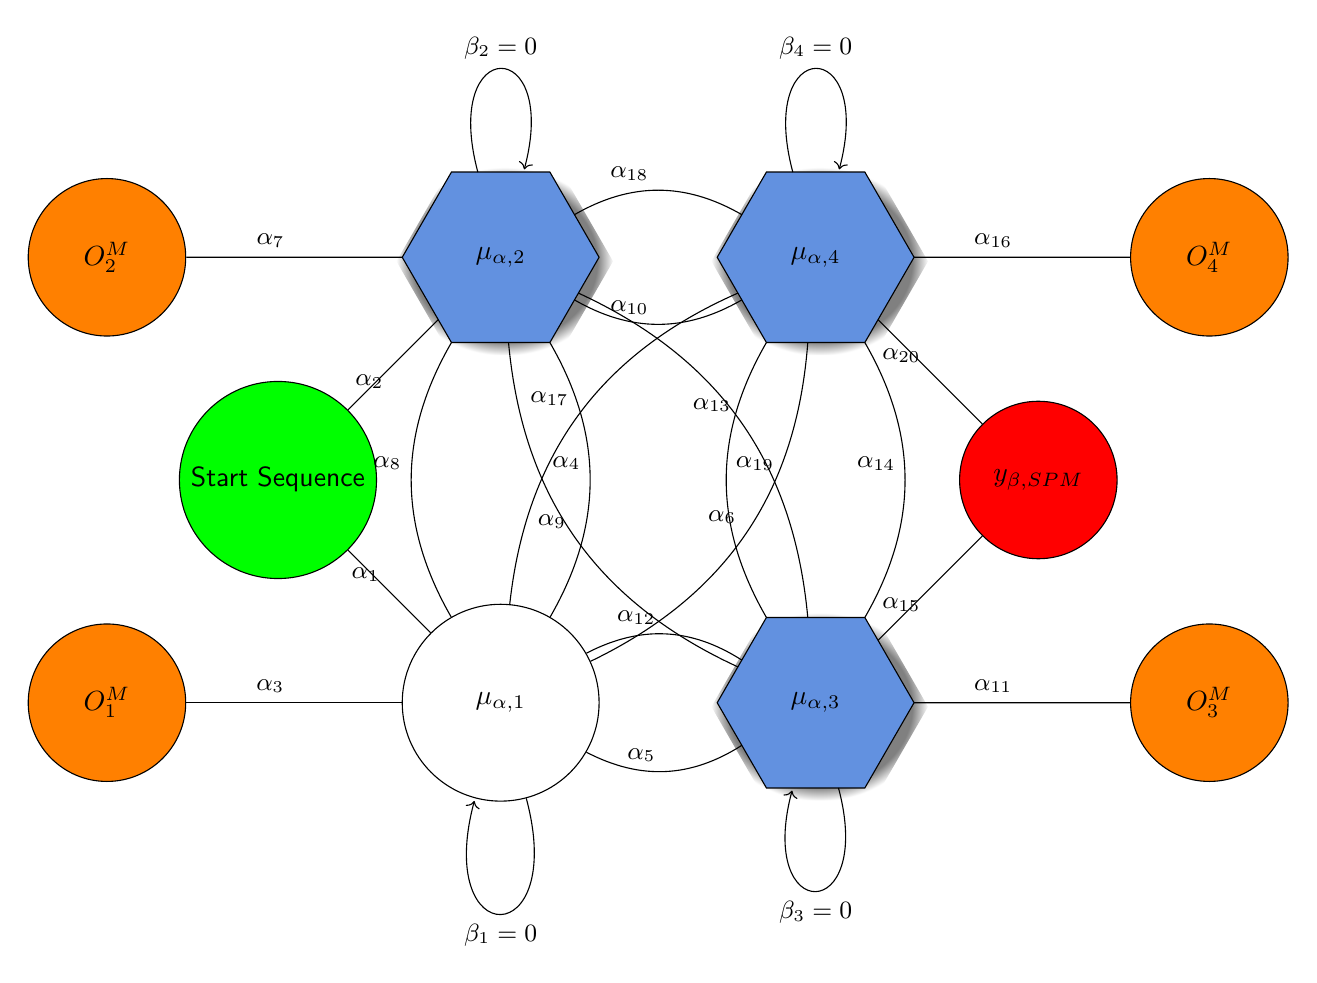
\begin{tikzpicture}

[->,>=stealth',shorten >=1pt,auto,node distance=4cm,
thick,main node/.style={circle,draw,font=\sffamily\Large\bfseries}]
\node[state,fill=green,minimum size=20mm,node distance=4cm] (1) {Start Sequence};
\node[state, minimum size=25mm,node distance=4cm] (2) [below right of=1]{$\mu_{\alpha,1}$};
\node[shapeHexagon,minimum size=25mm,node distance=4cm] (3)[above right of=1] {$\mu_{\alpha,2}$};
\node[shapeHexagon,minimum size=25mm,node distance=4cm] (4) [right of=2]{$\mu_{\alpha,3}$};
\node[shapeHexagon,minimum size=25mm,node distance=4cm] (5)[right of=3] {$\mu_{\alpha,4}$};
\node[state,fill=red,minimum size=20mm,node distance=4cm] (6) [above right of=4]{$y_{\beta,SPM}$};

\node[state,fill=orange,minimum size=20mm,node distance=5cm] (7) [left of=2]{$O_{1}^{M}$};
\node[state,fill=orange,minimum size=20mm,node distance=5cm] (8) [left of=3]{$O_{2}^{M}$};
\node[state,fill=orange,minimum size=20mm,node distance=5cm] (9) [right of=4]{$O_{3}^{M}$};
\node[state,fill=orange,minimum size=20mm,node distance=5cm] (10) [right of=5]{$O_{4}^{M}$};


\path[every node/.style={font=\sffamily\small}]
(1) edge [right] node[above left] {$\alpha_1$} (2)
(1) edge [right] node[below left] {$\alpha_2$} (3)

(2) edge [right] node[above left] {$\alpha_3$} (7)
(2) edge [bend right] node[above left] {$\alpha_4$} (3)
(2) edge [bend right] node[above left] {$\alpha_5$} (4)
(2) edge [bend right] node[above left] {$\alpha_6$} (5)
edge [loop below] node {$\beta_{1}=0$} (2)

(3) edge [right] node[above left] {$\alpha_7$} (8)
(3) edge [bend right] node[above left] {$\alpha_8$} (2)
(3) edge [bend right] node[above left] {$\alpha_9$} (4)
(3) edge [bend right] node[above left] {$\alpha_{10}$} (5)
edge [loop above] node {$\beta_{2}=0$} (3)

(4) edge [right] node[above left] {$\alpha_{11}$} (9)
(4) edge [bend right] node[above left] {$\alpha_{12}$} (2)
(4) edge [bend right] node[above left] {$\alpha_{13}$} (3)
(4) edge [bend right] node[above left] {$\alpha_{14}$} (5)
(4) edge [right] node[below  left] {$\alpha_{15}$} (6)
edge [loop below] node {$\beta_{3}=0$} (4)

(5) edge [right] node[above left] {$\alpha_{16}$} (10)
(5) edge [bend right] node[above left] {$\alpha_{17}$} (2)
(5) edge [bend right] node[above left] {$\alpha_{18}$} (3)
(5) edge [bend right] node[above right] {$\alpha_{19}$} (4)
(5) edge [right] node[above left] {$\alpha_{20}$} (6)
edge [loop above] node {$\beta_{4}=0$} (5)
;
\end{tikzpicture}

\end{document}
